\section{Differentialgleichungen}

\subsection{Lösen von Differentialgleichungen}

\subsubsection{Trennung von Variabeln \formelbuch{506}}
\begin{tabular}{p{4cm}p{1.5cm}p{10.5cm}}
\textbf{Form:} $y' = f(x) g(y)$ &
\textbf{Vorgehen:}              &
$\frac{y'}{g(y)} = f(x)$, nun ist die DGL beidseitig nach x integrierbar\\  &&
($dx = \frac{dy}{y'}$): $\int \frac{1}{g(y)} dy = \int f(x) dx$ 
\end{tabular}

\subsubsection{Lineartermsubstitution \formelbuch{506}}
\begin{tabular}{p{4cm}p{1.5cm}p{10.5cm}}
\textbf{Form:} $y'=f(ax+by+c)$   &
\textbf{Vorgehen:}               &
1. Substitution: $z=ax+by+c \qquad z'=a+by' =a+bf(z)$\\ &&
$\int\frac{z'}{a+bf(z)} = \int 1$
\end{tabular}

\subsubsection{Gleichgradigkeit}
\begin{tabular}{p{4cm}p{1.5cm}p{10.5cm}}
\textbf{Form:} $y'=f(\frac{y}{x})$ &
\textbf{Vorgehen:}                &
1. Substitution: $z=\frac{y}{x} \qquad
z'=\frac{1}{x}(f(z)-z)$
\end{tabular}

\subsubsection{Lineare Differentialgleichungen 1. Ordnung \formelbuch{507}}
\begin{tabular}{p{4cm}p{1.5cm}p{10.5cm}}
\textbf{Form:} $ y'+f(x)y = g(x) $ &
\textbf{Vorgehen:}                 &
$ y=e^{-\int f(x) dx}(k+\int g(x)e^{\int f(x)dx}dx)$
\end{tabular}

\subsection{Lineare Differentialgleichung 2. Ordnung mit konstanten 
Koeffizienten \formelbuch{525 ?}}
\begin{tabular}{p{8cm}p{8cm}}
\textbf{Form:} $y''+a_1\cdot y'+a_0\cdot y=f(x)$  &
\textbf{Störglied:} $f(x)$\\
\textbf{Homogene Differentialgleichung:} $f(x)=0$ &
\textbf{Inhomogene Differentialgleichung:} $f(x)\neq 0$
\end{tabular}

\subsubsection{Allgemeine Lösung einer homogenen DGL:\quad\subsubadd{$\quad Y_H$}}
\textbf{Charakteristisches Polynom}
$\qquad\underline{\lambda^2+a_1\cdot\lambda+a_0=0}$ \hspace{1cm}von
$\qquad\underline{y''+a_1\cdot y'+a_0\cdot y=0}$ 
$\qquad(\lambda_{1,2} = -\frac{a_1}{2} \pm \frac{\sqrt{a_1^2 - 4a_0}}{2})$\\ \\
\begin{tabular}{p{8cm}p{8cm}}
Falls $\lambda_1\neq \lambda_2$ und $\lambda_{1,2} \in R$:&
$Y_H=A_1e^{\lambda_1x}+A_2e^{\lambda_2x}$\\
Falls $\lambda_1=\lambda_2$ und $\lambda_{1,2} \in R$:    &
$Y_H=e^{\lambda_1x}(A_1+A_2\cdot x)$\\
Falls $\lambda_{1,2}=-\frac{a_1}{2}\pm j\alpha$:          &
$Y_H=e^{-\frac{1}{2}a_1x}(A_1cos(\alpha x) +A_2sin(\alpha x))$\\
\end{tabular}

\subsubsection{Allgemeine Lösung einer inhomogenen DGL:\quad\subsubadd{$y=Y_H+y_P$}}

\subsubsection{Grundlöseverfahren einer inhomogenen DGL:\quad\subsubadd{$\quad y_P$}}
Homogene DGL: $y''+a_1\cdot y'+a_0\cdot y=0$  für die  $g(x_0)=0$  und
$g'(x_0)=1$  gilt, ist:\\
$$y_P(x)=\int\limits_{x_o}^{x} g(x+x_0-t)\cdot f(t)dt$$\\
die partikuläre Lösung von $y''+a_1\cdot y'+a_0\cdot y=f(x)$

\subsubsection{Der Ansatz einer inh. DGL in Form des Störgliedes:\quad\subsubadd{$\quad y_P$}}
$f(x)=p_n(x)$\hspace{9cm}($p_n(x)$ und $q_n(x)$ sind Polynome vom gleichen Grad)\\
\begin{tabular}{p{8cm}p{4cm}}
Fall a: $a_0\neq 0$:          & $y_P = q_n(x)$\\
Fall b: $a_0 = 0 , a_1\neq 0$:& $y_P=x\cdot a_n(x)$\\
Fall c: $a_0=a_1=0$:          & $y_P=x^2\cdot q_n(x)$\\
\end{tabular}\\
$f(x)=e^{bx}\cdot p_n(x)$\\
\begin{tabular}{p{8cm}p{4cm}}
Fall a: $b$ nicht Nullstelle des char. Polynoms:    &
$y_P=e^{bx}\cdot q_n(x)$\\
Fall b: $b$ einfache Nullstelle des char. Polynoms: &
$y_P=e^{bx}\cdot x \cdot q_n(x)$\\
Fall c: $b$ zweifache Nullstelle des char. Polynoms:&
$y_P=e^{bx}\cdot x^2\cdot q_n(x)$\\
\end{tabular}

%%%%%%%%%%%%%%%%%%%%%%%%%%%%%%%%%%%%%%%%%%%%%%%%%%%%%%%%%%%%%%%%%%%%%%%%%%%%%%%%%%%%%%%%%%%%%%%%
%%%%%%%%%%%%%%%%%%%%%%%%%%%%%%%%%%%%%%%%%%%%%%%%%%%%%%%%%%%%%%%%%%%%%%%%%%%%%%%%%%%%%%%%%%%%%%%%

\newpage
\subsubsection{Superpositionsprinzip}
$f(x)=c_1f_1(x)+c_2f_2(x)$\\
\begin{tabular}{p{8cm}p{4cm}}
$y_1$ ist spezielle Lösung der DGL &
$y''+a_1\cdot y'+a_0\cdot y=c_1f_1(x)$ \\
$y_2$ ist spezielle Lösung der DGL &
$y''+a_1\cdot y'+a_0\cdot y=c_2f_2(x)$ \\
dann ist:                          &
$y_P=c_1y_1+c_2y_2$\\
\end{tabular}

\subsection{Lineare Differentialgleichung n. Ordnung mit konstanten 
Koeffizienten \formelbuch{?}}
\begin{tabular}{p{8cm}p{8cm}}
\textbf{Form:} &
$\sum\limits_{k=0}^na_ky^{(k)}= y^{(n)}+a_{n-1}\cdot y^{(n-1)}+\ldots +a_0\cdot y=f(x)$\\
\textbf{Algemeine Lösung der homogenen DGL:} &
$g=c_1g_1+c_2g_2+\ldots +c_kg_k$\\
\end{tabular}

\subsubsection{Homogene Lösungen}
\begin{tabular}{lll}
Fall a: r reelle Lösungen $\lambda_1$: 
  & $y_1=e^{\lambda_1x}$, $y_2=xe^{\lambda_1x}$, \ldots
  ,$y_r=x^{r-1}e^{\lambda_1x}$ 
  & Starke Dämpfung / Kriechfall\\
Fall b: $k$ komplexe Lösungen $\lambda_2=\alpha +j\beta$: 
  &$y_1=e^{\alpha x}\cos(\beta x)$, \ldots, $y_k=e^{\alpha x}x^{k-1}\cos(\beta
x)$
  & Schwache Dämpfung /\\
  &$y_{k+1}=e^{\alpha x}\sin(\beta x)$, \ldots, $y_{2k}=e^{\alpha
x}x^{k-1}\sin(\beta x)$
  & Schwingfall\\
\end{tabular}

\subsubsection{Allgemeinste Lösung des partikulären Teils:}
$$\underbrace{\sum_{k=0}^n a_k y^{(k)}}_{f(y,y',y'',\ldots)} = \underbrace{e^{\alpha x} (p_{m1}(x) \cos (\beta x) + q_{m2}(x) \sin (\beta x))}_{\text{Störglied}}$$
Unterscheide die Lösungen des charakteristischen Polynoms ($\lambda$):\hspace{5.5cm}mit m = max(m1, m2)\\
\begin{tabular}{p{8cm}p{8.5cm}}
Fall a: $\alpha + j\beta \neq \lambda$, so ist &
$y_P = e^{\alpha x}(r_m(x)\cos(\beta x) + s_m(x) \sin(\beta x))$\\
Fall b: $\alpha + j\beta$  ist u-fache Lösung von $\lambda$, so ist &
$y_P = e^{\alpha x} x^u (r_m(x) \cos(\beta x) + s_m(x) \sin(\beta x))$\\
&
u-fache Resonanz

\end{tabular}

\subsubsection{Grundlöseverfahren}
\begin{tabular}{p{12cm}p{5cm}}
$\begin{pmatrix}
g(x_0)=  & 0 & = & c_1g_1(x_0)+c_2g_2(x_0)+\ldots +c_n(x_0)\\
g'(x_0)= & 0 & = & c_1g_1'(x_0)+c_2g_2'(x_0)+\ldots +c_ng_n'(x_0)\\
\vdots  & \vdots & \\                            
g^{(n-1)}(x_0)= & 1 & = & c_1g_1^{(n-1)}(x_0)+c_2g_2^{(n-1)}(x_0)+\ldots
+c_ng_n^{(n-1)}(x_0)
\end{pmatrix}$ &
\begin{minipage}[t]{5cm}
ergibt $c_1,\ldots ,c_n$ für\\
$y_{P}(x)=\int_{x_0}^x{g(x+x_0-t)f(t)dt}$
\end{minipage}
\end{tabular}

\subsubsection{Hornerschema\formelbuch{914}}
\begin{minipage}[t]{9cm}
- Pfeile $\Rightarrow$ Multiplikation\\
- Zahlen pro Spalte werden addiert\\
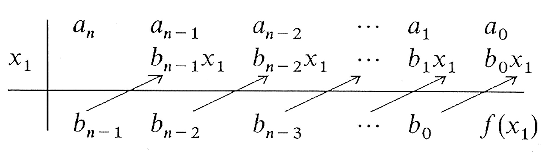
\includegraphics[width=6cm]{./bilder/Hornerschema_1.png}\\
$x_1 \Rightarrow$ Nullstelle (muss erraten werden!!)\\
oberste Zeile = zu zerlegendes Polynom
\end{minipage}
\begin{minipage}[t]{9cm}
\textbf{Beispiel:}\\
$f(x) = x^3-67x-126$\\
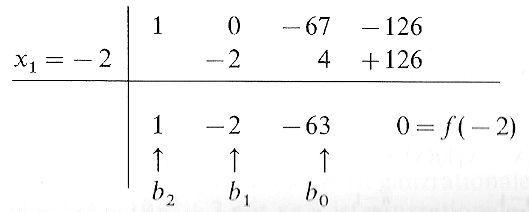
\includegraphics[width=6cm]{./bilder/Hornerschema_2.png}\\
$\Rightarrow f(x) = (x-x_1)(b_2x^2 + b_1x + b_0) = (x+2)(x^2-2x-63)$  
\end{minipage}

\subsection{Lineare Differentialgleichungssysteme erster Ordnung mit konstanten
Koeffizienten}
\begin{tabular}{p{8cm}p{8cm}}
\textbf{Form:}&
$\dot{x}=ax+by+f(t)$\\
&
$\dot{y}=cx+dy+g(t)$\\
\textbf{Die allgem. Lösung ergibt sich aus der DGL:}&
$\ddot{x}-(a+d)\dot{x}+(ad-bc)x=\dot{f}(t)-df(t)+bg(t)$\\
&
$y=\frac{1}{b}(\dot{x}-ax-f(t)))$\\
\end{tabular}
